\documentclass[11pt]{article}

% Prelude inclusion (packages and definitions).
\usepackage[a4paper,margin=1in]{geometry}
\usepackage[utf8]{inputenc}
\usepackage{graphicx}
\usepackage{minted}
\usepackage{stmaryrd}
\usepackage[english]{babel}
\usepackage{lmodern}
\usepackage{mathpazo}
\usepackage[T1]{fontenc}
\usepackage{forest}
\usepackage{caption}
\usepackage{subcaption}
\usepackage{fancyvrb}
\usepackage{hyperref}
\usepackage{appendix}
\usepackage{amssymb}
\usepackage{amsmath}
\usepackage{amsthm}
\usepackage{algorithm}
\usepackage[noend]{algpseudocode}
\usepackage{titlesec}
\usepackage[pdf]{graphviz}
\usepackage{titling}
\usepackage{enumitem}
\usepackage{tabu}
\usetikzlibrary{shapes,arrows}

% Custom figure captions
\DeclareCaptionFormat{customcap}{\vspace{0.5em}\linebreak\setlength{\fboxsep}{4pt}\colorbox{black!4}{\hspace{-0.1em}\parbox{0.98\linewidth}{\centering \textit{#1}#2#3}}\vspace{0.5em}}
\captionsetup[figure]{format=customcap}

% Custom appendix captions
\newcommand{\colorsection}[1]{%
  \vspace{0.5em}\linebreak\setlength{\fboxsep}{6pt}\colorbox{black!4}{\parbox{\linewidth}{\centering \textit{Appendix~\thesection}:\ #1}}\vspace{0.5em}}

% Highlight boxes
\def\highlightbox#1{\setlength{\fboxsep}{2pt}\colorbox{yellow!60}{\textbf{#1}}}

% Appendix reference boxes
\def\appendixref#1{\noindent\setlength{\fboxsep}{6pt}\colorbox{yellow!20}{$\hspace{0.3em} \triangleright$ \hspace{0.2em} \parbox{\linewidth-2.8em}{\textit{#1}}}}

% Title margins
\titlespacing*{\subsection}{0pt}{2\baselineskip}{\baselineskip}

% Algorithms formatting
\algrenewcommand\alglinenumber[1]{\footnotesize #1}
\algrenewcomment[1]{\(\triangleright\) #1}

% Circled numbers
\newcommand*\circled[1]{\tikz[baseline=(char.base)]{
    \node[shape=circle,draw,inner sep=2pt] (char) {#1};}}

% Subtitle definition
\newcommand*\subtitle[1]{\newcommand{\thesubtitle}{#1}}

% Credits definition
\newcommand*\credits[1]{\newcommand{\thecredits}{#1}}

% Abstract redefinition
\renewcommand\abstract[1]{\newcommand{\theabstract}{#1}}

% Theorems and definitions
\theoremstyle{definition}
\newtheorem{definition}{Definition}

\theoremstyle{plain}
\newtheorem{theorem}{Theorem}

% Asterisms
\newcommand{\asterism}{\smash{%
\raisebox{-.5ex}{%
\setlength{\tabcolsep}{-.5pt}%
\begin{tabular}{@{}cc@{}}%
\multicolumn2c*\\[-2ex]*&*%
\end{tabular}}}}

% Table of contents
\newcommand{\nocontentsline}[3]{}
\newcommand{\tocless}[2]{\bgroup\let\addcontentsline=\nocontentsline#1{#2}\egroup}

% Document metadata.
\title{Optimizing neural network inference on embedded devices}
\subtitle{And discovering the wonderful world of Rust in the process}
\credits{May-July 2018 -- at Snips Paris \\ Under the supervision of Mathieu Poumeyrol}
\author{Romain Liautaud}
\abstract{During my three-month internship in the Device Engineering team at Snips, I was tasked with improving the performance, efficiency and overall robustness of TFDeploy~\cite{tfdeploy}, their in-house port of TensorFlow inference to embedded devices. This report is a summary of this work, which involved topics ranging from static analysis and compiler optimizations to assembly programming.}

\begin{document}

% Front page inclusion.
\pagenumbering{gobble}
\newgeometry{vmargin=6em, hmargin=6em}
{\noindent
\large
Master in Computer Science \hfill Internship Report\\
\textit{École Normale Supérieure de Lyon} \hfill \textsc{\theauthor}}

\vspace{2.8em}

\hfuzz=5.002pt
\noindent
\setlength{\fboxsep}{15pt}
\colorbox{gray!20}{\parbox{\linewidth-30pt}{\raggedleft
    \vspace{2.5em}
    {\Large \textbf{\thetitle}} \\
    {\large \textit{\thesubtitle}}
}}

\vspace{2.5em}

\begin{center}
\textsc{\thecredits}
\end{center}

\vspace{1.3em}

\begin{center}
\parbox{0.84\linewidth}{
\setlength{\parindent}{11.1pt}
\noindent
\textsc{\textbf{Abstract}}\\

\theabstract
}
\end{center}

\vspace{1.3em}

\begin{center}
\parbox{0.84\linewidth}{
\setlength{\parindent}{11.1pt}
\noindent
\textsc{\textbf{Table of Contents}}

\vspace{-4em}
\renewcommand\contentsname{}
\tableofcontents}
\end{center}

\newpage
\pagenumbering{arabic}
\restoregeometry

\section*{Introduction}
\addcontentsline{toc}{section}{Introduction}

Snips is a french artificial intelligence startup which makes voice assistant solutions. Their voice assistants are not unlike Alexa, Siri or Google Home; except for two key differences:
\begin{itemize}
    \item First of all, they are entirely customize, meaning that the user can choose the hotword which will trigger the assistant~--~e.g. ``Hey Snips!''; the intents that the assistant will be able to understand; and the way the assistant will respond to these intents.
    
    \item And, most importantly, they are \textit{private by design}, meaning that they never send audio recordings of the user to a remote server for processing. This implies that the entire processing~--~which includes hotword detection, speech recognition, natural language understanding and speech synthesis~--~must happen directly on the device that recorded the audio, which can be anything from a PC or a smartphone to a Raspberry Pi.
\end{itemize}

To achieve this, Snips makes heavy use of machine learning and deep neural networks in particular: once the user has specified how he wants its assistant to behave, Snips trains several neural networks~--~for hotword recognition, speech recognition, natural language understanding, etc.~--~to match this behavior, and lets the user download these trained models on their device so that they can be run there.\\

One of the tasks of the Device Engineering team, in which I was doing my internship, is to make sure that these pre-trained models run as well as possible on embedded devices such as smartphones or single-board computers like the Raspberry Pi. Indeed, these devices are usually limited in computing power, memory and disk space; and some of them run even run on batteries, making energy efficiency an important factor.

However, most of the many open source machine learning libraries available online were not designed with embedded devices in mind, but rather with data centers and giant clusters of high-powered GPU machines. For instance, when compiled, the TensorFlow~\cite{tensorflow} library embarks code to both train and infer~--~i.e. evaluate~--~neural networks on CPUs and GPUs; and so the library takes way too much time to compile and too much disk space for what is actually needed: inference on tiny CPUs.\\

There have been several initiatives to improve this situation:
\begin{itemize}[noitemsep]
    \item There is now a separate, trimmed-down build of TensorFlow \cite{tensorflow-mobile} for smartphones;
    \item There are attempts at using ahead-of-time compilation \cite{tensorflow-aot} and just-in-time compilation \cite{tensorflow-jit} to improve the inference speed of neural network models expressed with TensorFlow;
    \item More recently, Google has released a preview of TensorFlow Lite \cite{tensorflow-lite}, an inference-only subset of TensorFlow optimized for embedded devices.
\end{itemize}

One of these initiatives is TFDeploy~\cite{tfdeploy}, a TensorFlow-compatible inference library for embedded devices written by Snips' Device Engineering team in Rust~\cite{rust}, a new systems programming language which promises to be as fast as C or C++ while preventing segfaults; guaranteeing thread safety; providing powerful abstractions~--~like a ML-based type system with pattern matching, or iterators~--~without runtime costs; and much more.

TFDeploy was designed with several goals in mind: first, the compiled inference runtime should take up as little disk space as possible; and the library should also help reduce the disk space used by pre-trained models. On a given model, TFDeploy inference should run as fast as TensorFlow inference; and ideally faster~--~by optimizing the inference code for architectures like ARM. My task, during this internship, was to help TFDeploy meet these goals. 

In this report, I will present a static analyser for dataflow graphs which helped reduce the disk space and inference time of pre-trained models; as well as new inference semantics which helped avoid redundant computations when dealing with streamed~--~e.g. audio~--~input data.

\newpage
\subsection*{TensorFlow and its dataflow graph.}

Among the many open source deep learning libraries available online, TensorFlow~\cite{tensorflow} is by far the most popular~--~with more than 100,000 stars on GitHub at the time of writing. Under active development by Google since 2015, it lets developers define, train and evaluate most types of deep neural networks~--~including convolutional and recurrent networks~--~but can also be used more generally as a framework for high performance numerical computation.

But, more than the library itself, we're actually mainly interested TensorFlow's internal representation of neural networks and numerical computations in general: the \textbf{dataflow graph}. As explained in the TensorFlow documentation \cite{tensorflow-doc-graph}, this graph is used to represent any computation in terms of the dependencies between individual operations~--~e.g. element-wise matrix operations, matrix products or 2-D convolutions. As an example, Fig.~\ref{fig-example-perceptron} shows the dataflow graph of a single-layer perceptron.

\bigskip
\begin{figure}[!h]
    \caption{Dataflow graph of a single-layer perceptron with bias and ReLU activation.}
    \label{fig-example-perceptron}
    \vspace{-1.5em}
    \hspace*{-6.4em}
    \includegraphics[width=1.3\textwidth]{example-perceptron.pdf}
    \vspace{-2em}
\end{figure}

Let us start by formalizing this internal representation. In TensorFlow, the basic unit of computation is the \textbf{tensor}, which is essentially a generalization of vectors and matrices to any dimension and datatype.\\

\begin{definition}
A \textbf{tensor} $t \in \mathcal{T}$ is an $n$-dimensional array of scalars, with $n \in \mathbb{N}$.\\

Every tensor has the following properties:
\begin{itemize}[noitemsep]
    \item A \textbf{datatype}, e.g. \texttt{float32} or \texttt{uint8}, which is shared by all the scalars inside the tensor;
    \item A \textbf{rank}, which is the dimensionality of its underlying array (here the integer $n$);
    \item A \textbf{shape}, which is an $n$-tuple of integers that represents the size of each dimension.
\end{itemize}

 \textit{Note that a $0$-ranked tensor, or equivalently a tensor with shape \texttt{()}, is simply a scalar.}\\
\end{definition}

\begin{definition}
A \textbf{dataflow graph} $G = (V_G,\ E_G,\ op,\ n_i,\ n_o,\ a)$ is a directed acyclic multigraph.

\textit{Note that, in the general case, dataflow graphs are not necessarily acyclic; but since the scope of this report~--~and this internship~--~is limited to convolutional neural networks, we will make the simplifying assumption that they don't contain any cycles.}\\

Every node in $v \in V$ has:
\begin{itemize}[noitemsep]
    \item An operation $op(v)$, e.g. \texttt{Const}, \texttt{Add} or \texttt{Conv2D}, which defines the behavior of the node;
    \item A map $a(v)$ of attributes with keys from the set $\mathcal{A}_{op(v)}$ of possible keys for the operation;
    \item A set of $n_i(v)$ input ports and $n_o(v)$ output ports;
\end{itemize}

Some nodes have the special \texttt{Placeholder} operation, which is not an actual operation but instead a way to mark the nodes which will be replaced by the input data before inference.\\

Every edge $e \in E$ is a tuple $(v_s,\ p_s,\ v_d,\ p_d)$ with $v_s$ and $v_d$ the source and destination nodes of the edge respectively, $p_s \in \llbracket 0,\ n_o(v_s) \llbracket$ the output port of the source node and $p_d \in \llbracket 0,\ n_i(v_d) \llbracket$ the input port of the destination node used by the edge.\\

For convenience, let us define the incoming and outgoing edges of a node as:

\noindent\begin{minipage}{.5\linewidth}
    \begin{equation*}
    e_i(v) = \bigcup_{p = 0}^{n_i(v)} e_i(v, p)
    \end{equation*}
\end{minipage}%
\begin{minipage}{.5\linewidth}
    \begin{equation*}
    e_o(v) = \bigcup_{p = 0}^{n_o(v)} e_o(v, p)
    \end{equation*}
\end{minipage}

\vspace{.5em}
\noindent
with the incoming \textit{(resp. outgoing)} edges to \textit{(resp. from)} an input \textit{(resp. output)} port of a node as:
\begin{align*}
    e_i(v, p) &= \{(v_s,\ p_s,\ v,\ p) \in E\ |\ v_s \in V,\ p_s \in \llbracket 0,\ n_o(v_s) \llbracket \}\\
    e_o(v, p) &= \{(v,\ p,\ v_d,\ p_d) \in E\ |\ v_d \in V,\ p_d \in \llbracket 0,\ n_i(v_d) \llbracket \}\\
\end{align*}
\end{definition}

Let us now model the semantics of TensorFlow inference. Essentially, the semantics of every operation is given by its evaluation function, which takes a set of attribute values and a set of input tensors, and returns a set of output tensors. Running inference on a dataflow graph is then just a matter of finding an execution plan, replacing the \texttt{Placeholder} nodes with the input data, and, for every node in the plan, applying the evaluation function of its operation on the tensors of its input ports and putting the result on its output ports.\\

\begin{definition}Every operation $op$ is associated with an \textbf{evaluation function}:
$$eval_{op} \ :\ \mathcal{P}(\mathcal{A}_{op})\ \times \ \mathcal{T}^{n_i} \ \rightarrow \mathcal{T}^{n_o}$$
with $n_i$ and $n_o$ respectively the number of input and output ports that $op$ expects.\\

\noindent
Here are several examples of evaluation functions:
\begin{itemize}
    \item $eval_\texttt{Const}(attrs,\ ()) = attrs[\texttt{value}]$ (i.e. the value associated with the key \texttt{value} in $attrs$);
    \item $eval_\texttt{Add}(attrs,\ (a, b)) = (a + b)$ (with $a + b$ the element-wise sum of tensors $a$ and $b$);
    \item $eval_\texttt{AddN}(attrs,\ inputs) = \left( \sum_{i = 0}^{attrs[\texttt{n}]} inputs[i] \right)$\\ \textit{Note how the operation can handle a variable number of inputs via the \texttt{n} attribute.}\\
\end{itemize}
\end{definition}

\begin{definition}
An \textbf{execution plan} for a dataflow graph $G$ with output node $v^* \in V_G$, if it exists, is a topological ordering $ord$ of $(V_G, \overline{E_G})$ such that: $$\forall v \in V,\ op(v)\ =\ \texttt{Placeholder} \Rightarrow ord(v) <= ord(v^*)$$ With $\overline{E}$ the set of edges without the input and output port information: $$\overline{E} = \{(v_s,\ v_d)\ \in V \times V |\ \exists p_s \in \llbracket 0,\ n_o(v_s) \llbracket,\ p_d \in \llbracket 0,\ n_i(v_d) \llbracket,\ (v_s,\ p_s,\ v_d,\ p_d) \in E\}$$
\end{definition}

\bigskip
\begin{definition}
The \textbf{inference function} $infer_G\ : \ V_G \times \mathcal{T} \rightarrow \mathcal{T}$ of a dataflow graph $G$ is defined as the return value of the following algorithm, which takes an output node $v^* \in V_G$ and an input tensor $t^* \in \mathcal{T}$, and returns the result at $v^*$ of the computation described by $G$ in $O(V_G + E_G)$ \textit{(ignoring the complexity of computing the different evaluation functions)}.\\

\begin{algorithmic}[1]
\Function{InferGraph}{$G,\ v^*,\ t^*$}
    \State $ord \gets \textsc{ComputePlan}(G,\ v^*)$\\
    
    \State \Comment{We tag each edge of $G$ with a tensor (which doesn't yet have a value).}
    \State $tensors \gets [\texttt{null} \textbf{ for } e \in E]$\\
    
    \For{$v \in ord$}
        \If{$op(v) = \texttt{Placeholder}$}
            \For{$e \in e_o(v)$}
                \State $tensors[e] \gets t^*$
            \EndFor
        \Else
            \State $inputs \gets [tensors[e] \texttt{ for } e \in e_i(v)]$
            \State $outputs \gets eval_{op(v)}(a(v),\ inputs)$\\
            
            \State \Comment{The $eval$ function returns a tuple of tensors, one for each output port.}
            \For{$output \in outputs$}
                \State $p \gets index(output,\ outputs)$
                \For{$e \in e_o(v, p)$}
                    \State $tensors[e] \gets output$
                \EndFor
            \EndFor
        \EndIf\\

        \State \Comment{When we reach the output node, return its outgoing tensors.}
        \If{$v = v^*$}
            \State \Return $[tensors[e] \texttt{ for } e \in e_o(v)]$
        \EndIf
    \EndFor
\EndFunction
\end{algorithmic}

\end{definition}

\newpage
\section{Profiling and visualization tools}

Although I already clarified what we meant by ``\textit{optimizing} inference``~--~we wanted to make it faster, more energy- and space-efficient and more robust~--~I didn't specify how we were planning on doing that. The reason is simple: we didn't actually know, in the beginning, which part of the inference process could be optimized. We had hunches, of course, but we didn't want to act on them without proof to avoid premature optimization.

Consequently, we needed a proper set of tools to visualize dataflow graphs and profile their inference on both TFDeploy \cite{tfdeploy} and the reference TensorFlow implementation \cite{tensorflow}; and that is what I did during the first few weeks of my internship. Although it was not really scientifically challenging work, it helped me get familiar with the TFDeploy codebase and with Rust \cite{rust}~--~the programming language it's written in~--~whose memory ownership model is a bit unsettling at first. In hindsight, spending time writing these tools first also saved me a lot of time in the long run, as I was able to work much faster using them.

\subsection{Command-line profiler.}
I started by writing a command-line interface \cite{cli} that allowed me to, among other things, display general information about a dataflow graph, profile the execution of a graph using randomly generated data, or compare the values returned by TFDeploy and the reference implementation to check for correctness. Fig.~\ref{fig-tfdeploy-profiler} shows an excerpt of the command-line output when profiling the execution of a graph. Notice how we distinguish the \textit{real} time~--~which is the actual time elapsed, as measured by a clock on the wall~--~from the \textit{user} and \textit{sys} times~--~which correspond to the amount of CPU time spent in user-mode code and kernel calls respectively. This distinction was useful to pinpoint what exactly was taking up time, especially in multi-threaded contexts.

\bigskip
\begin{figure}[!h]
\centering
    \caption{Partial output of the \texttt{./cli conv2d.pb -s 61x60xf32 profile} command.}
    \label{fig-tfdeploy-profiler}
    \vspace{-.2em}
    \includegraphics[width=0.9\textwidth]{tfdeploy-profiler.png}
    \vspace{-1em}
\end{figure}

Getting accurate measurements was actually harder than I expected: as most of the events that I had to profile were taking less than $20$~ms (sometimes down to $0.01$~ms), slight variations in CPU clock rate~--~e.g. because of throttling~-- or even the measurement code itself could have a noticeable impact on the results. This was solved by adding a number of ``warm-up iterations'' that weren't measured but forced the CPU out of throttling, as well as measuring enough iterations to detect and remove outliers.

\subsection{Dataflow graph visualizer.}
After playing around with a few real-world CNN~--~convolutional neural network~--~models that the Snips hotword recognition team provided me~--~with more than $3000$ nodes for some of them~--~I realized that I needed a better way to visualize dataflow graphs than a simple Graphviz output. Drawing inspiration from TensorBoard~\cite{tensorboard}~--~which was unfortunately incompatible with the graph format used by TFDeploy~--~I wrote a visualization tool \cite{visualizer} which:
\begin{itemize}[noitemsep]
    \item allows you to group related parts of the graph and collapse them for better readability;
    \item shows the properties of nodes and edges;
    \item displays the hints provided by the static analyser \textit{(see Sec.~\ref{sec-static})}.
\end{itemize}

Although there are many existing graph layout algorithms to choose from, such as \cite{dag-algorithm} which is famously used by Graphviz or \cite{force-algorithm} which simulates a set of repulsive and attractive forces and tries to find a stable equilibrium, none of them gave me satisfying results~--~as Appendix~\ref{appendix-graphviz} demonstrates. So I decided to design one specifically for displaying dataflow graphs~--~which are essentially directed acyclic graphs with a few subtleties depending on the type of each node. To this end, I translated my graph layout problem into a set of linear constraints on the $x$ and $y$ coordinates of each node in the graph, which I then solved using a Javascript implementation \cite{kiwi-js} of the Cassowary constraint solving algorithm \cite{cassowary}. Fig.~\ref{fig-tfdeploy-visualizer} shows the output of the visualizer on the same model as in Appendix~\ref{appendix-graphviz}.

\bigskip
\begin{figure}[!h]
\centering
    \caption{Output of the visualizer on a hotword detection model used at Snips.}
    \label{fig-tfdeploy-visualizer}
    \vspace{-1.4em}
    \includegraphics[width=0.92\textwidth]{tfdeploy-visualizer.png}
    \vspace{-4em}
\end{figure}

\restoregeometry
\newpage
\section{Static analysis of dataflow graphs}
\label{sec-static}

My first \textit{actual} task was formalizing and implementing a \textbf{static analyser} for dataflow graphs, drawing inspiration from the abstract interpretation formalism \textit{(see \cite{roux-book} and \cite{schwartzbach-notes})}. This came as the natural answer to several problems:

\begin{itemize}
    \item First, the error messages displayed by TFDeploy were not explicit enough, for instance when the shape of the input data was incompatible with the shapes that the operations in the graph expected;
    \item What's more, all these errors were triggered at runtime, and we wanted a way to catch as many of them as possible ahead of time to avoid unpredictable runtime behavior;
    \item We also wanted to improve the graph visualization tool \cite{visualizer} that I mentioned earlier by annotating edges with information about the tensors flowing through them~--~e.g. their datatype, shape and value;
    \item Finally, we needed a framework on top of which we could build ahead-of-time optimizations like constant folding and propagation.
\end{itemize}

Simply put, the role of this analyser is to tag every edge in the graph with invariants about the tensors that flow through it~--~specifically their datatype, their shape and possibly their value. To do so, we will supplement each TensorFlow operation with a set of rules that express constraints on the datatype, shape and value of its input and output tensors; and we will then propagate those constraints~--~along with constraints about the input of the model~--~to the entire graph until we find those invariants.

In the following sections, I will give a formal overview of the analyser; describe the propagation algorithm used to find the edge invariants; present the declarative solver that I designed to help express constraints about the input and output tensors of operations; and quickly present some of the optimizations that I was able to implement using this static analyser.

\subsection{Formal overview.}

As we want to tag the edges of the dataflow graph with invariants about tensors, we must first formalize what these invariants can be. Here are a few of the things we might want to express:
\begin{itemize}[noitemsep]
    \item Every tensor flowing through this edge has datatype \texttt{float32};
    \item Every tensor flowing through this edge has shape $(2, 2)$;
    \item Every tensor flowing through this edge has rank $2$;
    \item Every tensor flowing through this edge has rank $2$ or more and its first dimension is $5$;
    \item Every tensor flowing through this edge has the same value of $t$.
\end{itemize}

To do so, we first define datatype, shape, value and ultimately tensor \textbf{facts}. They are analogous to the abstract values that are used in abstract interpretation.

\bigskip
\begin{definition}
A \textbf{datatype fact} $f \in \mathcal{TF}$ is either:
\begin{itemize}[noitemsep]
    \item $\top_\mathcal{TF}$, which matches any possible datatype;
    \item $Only_\mathcal{TF}(T)$ for $T$ a datatype, which only matches a specific datatype \textit{(e.g. $Only_\mathcal{TF}(\texttt{float32})$)};
    \item $\bot_\mathcal{TF}$, which signifies an error.
\end{itemize}

In the code, $\top_\mathcal{TF}$ is called \texttt{TypeFact::Any} and $Only_\mathcal{TF}(T)$ is called \texttt{TypeFact::Only}.\\
\end{definition}

\begin{definition}
A \textbf{value fact} $f \in \mathcal{VF}$ is either:
\begin{itemize}[noitemsep]
    \item $\top_\mathcal{VF}$, which matches any possible tensor;
    \item $Only_\mathcal{VF}(t)$ for $t$ a tensor, which only matches a specific tensor;
    \item $\bot_\mathcal{VF}$, which signifies an error.
\end{itemize}

In the code, $\top_\mathcal{VF}$ is called \texttt{ValueFact::Any} and $Only_\mathcal{VF}(t)$ is called \texttt{ValueFact::Only}.\\
\end{definition}

\begin{definition}
A \textbf{shape fact} is an element of $\mathcal{SF} \equiv \{0,\ 1\} \times \left(\mathbb{N} \cup \{\_\}\right)^*$. The first element defines whether the shape is \textit{closed} or \textit{open}, and the second element is a sequence of either an integer~--~which matches a specific dimension~--~or ``$\_$''~--~which matches any dimension.

For the sake of readability, we will write closed shape facts like regular sequences, and open shape facts with ``\texttt{..}'' in the end. While closed shape facts match an entire shape, an open shape fact only matches the beginning of a shape. So, for instance, the closed shape fact \texttt{[1, \_]} only matches the shapes $(1,\ k)$ with $k \in \mathbb{N}$, whereas the open shape fact \texttt{[1, \_, ..]} matches $(1,\ k)$ with $k \in \mathbb{N}$ as well as $(1,\ k,\ k')$ with $k, k' \in \mathbb{N}$, and so on.\\

This definition is a bit trickier than the previous ones, but is necessary to represent partial rank and shape information with enough precision. Looking back at our examples:
\begin{itemize}[noitemsep]
    \item ``Every tensor has shape $(2, 2)$'' can be represented by \texttt{[2, 2]};
    \item ``Every tensor has rank $2$'' can be represented by \texttt{[\_, \_]};
    \item ``Every tensor has rank $\geq 2$ and first dimension $5$'' can be represented by \texttt{[5, \_, ..]}.\\
\end{itemize}
\end{definition}

\begin{definition}
A \textbf{tensor fact} is an element of $\mathcal{F} \equiv \mathcal{TF} \times \mathcal{SF} \times \mathcal{VF}$.\\
\end{definition}

Now that we have a way to represent partial information (i.e. invariants) about tensors, we need to define a few well-chosen orders $\sqsubseteq_\mathcal{TF}$, $\sqsubseteq_\mathcal{SF}$, $\sqsubseteq_\mathcal{VF}$ and ultimately $\sqsubseteq_\mathcal{F}$ on our facts to give them a lattice structure. For the sake of clarity, we will not do that formally, but rather give excerpts of the Hasse diagrams for $\mathcal{TF}$, $\mathcal{SF}$ and $\mathcal{VF}$ on Fig.~\ref{fig-analyser-hasse}, and define that $(t_1,\ s_1,\ v_1) \sqsubseteq_\mathcal{F} (t_2,\ s_2,\ v_2)$ iff. $t_1 \sqsubseteq_\mathcal{TF} t_2$, $s_1 \sqsubseteq_\mathcal{SF} s_2$ and $v_1 \sqsubseteq_\mathcal{VF} v_2$.\\

\begin{figure}[!h]
\centering
    \caption{Hasse diagrams for $\mathcal{TF}$, $\mathcal{SF}$ and $\mathcal{VF}$.}
    \label{fig-analyser-hasse}
    \begin{minipage}{.5\linewidth}
        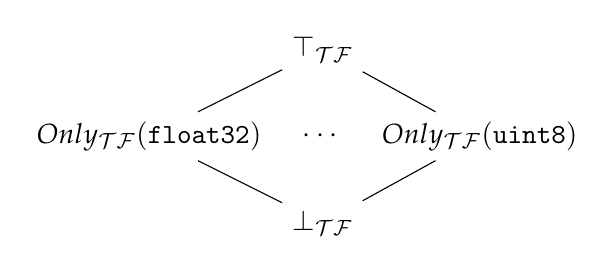
\begin{tikzpicture}
          \node (top) at (0,0) {$\top_\mathcal{TF}$};
          \node (a) at (-2.2,-1.1) {$Only_\mathcal{TF}(\texttt{float32})$};
          \node (dots) at (0,-1.1) {$\cdots$};
          \node (d) at (2,-1.1) {$Only_\mathcal{TF}(\texttt{uint8})$};
          \node (bot) at (0,-2.2) {$\bot_\mathcal{TF}$};
          \draw (top) -- (a) -- (bot) -- (d) -- (top);
        \end{tikzpicture}
        \vspace{-1.3em}
    \end{minipage}%
    \begin{minipage}{.5\linewidth}
        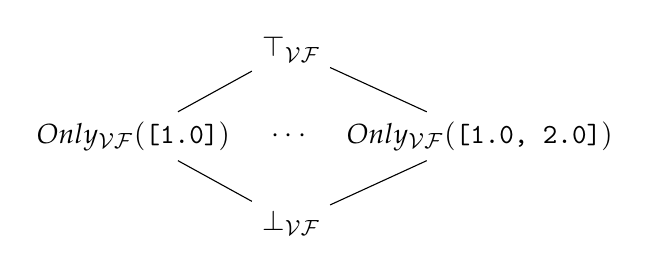
\begin{tikzpicture}
          \node (top) at (0,0) {$\top_\mathcal{VF}$};
          \node (a) at (-2,-1.1) {$Only_\mathcal{VF}(\texttt{[1.0]})$};
          \node (dots) at (0,-1.1) {$\cdots$};
          \node (d) at (2.4,-1.1) {$Only_\mathcal{VF}(\texttt{[1.0, 2.0]})$};
          \node (bot) at (0,-2.2) {$\bot_\mathcal{VF}$};
          \draw (top) -- (a) -- (bot) -- (d) -- (top);
        \end{tikzpicture}
        \vspace{-1.3em}
    \end{minipage}
    \hspace*{-10em}
    \vspace*{-1em}
    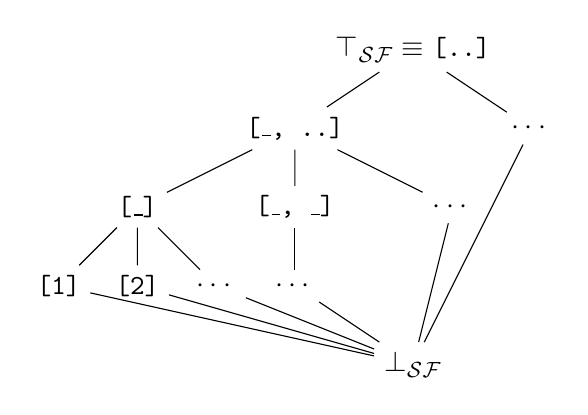
\begin{tikzpicture}
      \node (top) at (0,0) {$\top_\mathcal{SF} \equiv \texttt{[..]}$};
      \node (a1) at (-1.5,-1) {\texttt{[\_, ..]}};
      \node (ad) at (1.5,-1) {$\cdots$};
      \node (b1) at (-3.5,-2) {\texttt{[\_]}};
      \node (b2) at (-1.5,-2) {\texttt{[\_, \_]}};
      \node (bd) at (0.5,-2) {$\cdots$};
      \node (c1) at (-4.5,-3) {\texttt{[1]}};
      \node (c2) at (-3.5,-3) {\texttt{[2]}};
      \node (cd) at (-2.5,-3) {$\cdots$};
      \node (ed) at (-1.5, -3) {$\cdots$};
      \node (bot) at (0,-4) {$\bot_\mathcal{SF}$};

      \draw (a1) -- (top) -- (ad);
      \draw (b1) -- (a1) -- (b2);
      \draw (bd) -- (a1);
      \draw (c1) -- (b1) -- (c2);
      \draw (cd) -- (b1);
      \draw (ed) -- (b2);
     
      \draw (ad) -- (bot) -- (bd);
      \draw (cd) -- (bot) -- (ed);
      \draw (c1) -- (bot) -- (c2);
    \end{tikzpicture}
\end{figure}

\begin{definition}
For a lattice $L$, we finally define the \textbf{unification} of $a, b \in L$, written as $a \sqcap_L b$, as the largest $c \in L$ such that $c \sqsubseteq_L a$ and $c \sqsubseteq_L b$ \textit{(which always exists in a lattice)}.

In other words, $a \sqcap_L b$ is the most general fact that combines the information from both $a$ and $b$~--~it can be $\bot_L$ if $a$ and $b$ are incompatible facts. For instance:
$$
\begin{tabu}{rcll}
\top_\mathcal{TF} & \sqcap_\mathcal{TF} & Only_\mathcal{TF}(\texttt{float32}) &=
    Only_\mathcal{TF}(\texttt{float32})\\
Only_\mathcal{VF}(\texttt{[1]}) & \sqcap_\mathcal{VF} & Only_\mathcal{VF}(\texttt{[2]}) &=
    \bot_\mathcal{TF} \\
\texttt{[1, \_, ..]} & \sqcap_\mathcal{SF} & \texttt{[\_, \_, 3]} &=
    \texttt{[1, \_, 3]}
\end{tabu}
$$
\end{definition}

In practise, we don't actually implement the lattices themselves, but directly the unification functions. These functions, along with the Rust type definitions for \texttt{TypeFact}s, \texttt{ShapeFact}s, \texttt{ValueFact}s and \texttt{TensorFact}s, can be found on Appendix~\ref{appendix-analyser-types}. Note that we never directly encounter $\bot$ in the code, but raise an error as soon as the $\bot$ value would be produced.

\subsection{At the graph level: propagation algorithm.}

Using the above formalism, we can now describe the propagation algorithm used to find the edge invariants. Essentially, we start by tagging every edge of the graph with $\top_\mathcal{TF}$~--~the most general tensor fact possible. Then, in turn, each node in the graph adds more constraints to the tensor facts of its incoming and outgoing edges~--~we call this operation \textit{enrichment}~--~until reaching a fixed point.\\

\begin{definition}
We implement, for each operation $op$, an \textbf{enrichment function}:
$$enrich_{op} \ : \ \mathcal{P}(\mathcal{A}_{op}) \times \mathcal{F}^{n_i} \times \mathcal{F}^{n_o} \rightarrow \mathcal{F}^{n_i} \times \mathcal{F}^{n_o}$$
with $n_i$ and $n_o$ respectively the number of input and output ports that $op$ expects. This function takes the attributes of a node as well as the current facts about the node's input and output tensors, and returns an enriched~--~i.e. more precise~--~set of facts.\\
\end{definition}

That gives us the following algorithm, with $hints \in \mathcal{P}(V_G \times \mathcal{F})$ a set of hints to give to the analyser, which is useful if we already know the shape of the input data for instance.\\

\begin{algorithmic}[1]
\Function{AnalyseGraph}{$G,\ hints$}
    \State $ord \gets \textsc{ComputePlan}(G,\ v^*)$\\
    
    \State \Comment{We tag each edge of $G$ with a tensor fact (which is the most general for now).}
    \State $facts \gets [\top \textbf{ for } e \in E]$\\

    \State \Comment{We use the given hints to add more information to the edges.}
    \For{$(v, fact) \in hints$}
        \For{$e \in e_o(v)$}
            \State $facts[e] \gets facts[e] \sqcap fact$
        \EndFor
    \EndFor\\
    
    \State \Comment{We propagate the facts until reaching a fixed point.}
    \Loop
        \State $changed \gets \texttt{false}$\\

        \For{$v \in ord$}
            \State $inputs \gets [facts[e] \texttt{ for } e \in e_i(v)]$
            \State $outputs \gets [facts[e] \texttt{ for } e \in e_o(v)]$\\
            
            \State $(\overline{inputs},\ \overline{outputs}) \gets enrich_{op(v)}(a(v),\ inputs,\ outputs)$\\
            
            \For{$fact \in \overline{inputs}$}
                \State $p \gets index(fact,\ \overline{inputs})$
                \For{$e \in e_i(v, p)$}
                    \State $facts[e] \gets facts[e] \sqcap fact$
                \EndFor
            \EndFor\\
            
            \For{$fact \in \overline{outputs}$}
                \State $p \gets index(fact,\ \overline{outputs})$
                \For{$e \in e_o(v, p)$}
                    \State $facts[e] \gets facts[e] \sqcap fact$
                \EndFor
            \EndFor
        \EndFor\\
        
        \State $ord \gets reverse(ord)$\\

        \If{$\neg changed$}
            \State \Return $facts$
        \EndIf
    \EndLoop
\EndFunction
\end{algorithmic}

\bigskip
This algorithm roughly corresponds to the chaotic iterations algorithm from traditional static analysis. Let $n \equiv |V_G|$, $e \equiv |E_G|$, $h$ the height of the lattice $\mathcal{F}$, and $c$ the cost \textit{(which we assume is the same for every operation)} of calling $enrich_{op(v)}$ and $\sqcap$. In the worst case, in each iteration of the outer loop, only one edge of one node would get a tiny bit more information \textit{(but each of the $n$ nodes would make a call to $enrich_{op(v)}$ and $\sqcap$)}, giving us a complexity of $O(n * c * e * h)$.\\

This worst-case complexity, however, is far from realistic. One way to improve the practical performance of the algorithm is to use a well-chosen heuristic for the order in which nodes are picked in the inner loop. Here, as you can see on lines \texttt{17} and \texttt{33}, we start by propagating the information forward~--~w.r.t. the execution plan~--~then backward, then forward, etc.

The intuition behind this is that we'll start by propagating information about the \texttt{Placeholder} nodes \textit{(that we get from the $hints$)} to the rest of the graph, and along the way the nodes will add more constraints about the inputs and outputs, which we'll use on our way back up, etc. Using this heuristic, I was able to get down the number of outer loop iterations to at most 4 on all the real-world graphs I tested.\\

\bigskip
\appendixref{The Rust implementation of the propagation algorithm can be found in Appendix~\ref{appendix-analyser-algorithm}.}

\subsection{At the operation level: declarative constraint solver.}

There is still a problem, though: we must now write the $enrich_{op}$ function for every operation, and the task is much more cumbersome than it seems~--~especially considering that TFDeploy supports more than $20$ different operations.\\

My first attempt at tackling that problem was to implement two simpler functions for every operation: ${enrich^\rightarrow}_{op}$ and ${enrich^\leftarrow}_{op}$. The first one, called \textit{forward enrichment}, would only return a new set of output facts given a node's current input facts; and the second one, called \textit{backward enrichment}, would do the opposite. Even though that doubled the number of functions to implement, they were simpler to write (\url{https://github.com/kali/tensorflow-deploy-rust/tree/33b48389aecd20262cc16056af9b1e3f7c8a53f0} shows what the code looked like using this approach). But, after spending more than a week implementing all these functions, I was still not satisfied.

First of all, the separation into forward and backward enrichment reduced the accuracy of the static analyser. Take the \texttt{Pad} operation \cite{tensorflow-pad} for instance: it has two input ports called \texttt{input} and \texttt{paddings}, one output port called \texttt{output}, and it pads the beginning and end of each dimension of \texttt{input} with a number of zeros specified in \texttt{paddings}. So, if we have information about the value of \texttt{paddings} and the shape of \texttt{output}, we might be able to deduce the shape of \texttt{input}; but this is impossible to express when forward and backward enrichment are separated.

An even bigger problem was that ${enrich^\rightarrow}_{op}$ and ${enrich^\leftarrow}_{op}$ were still cumbersome to write~--~no matter how many helper functions and macros I tried to throw at the problem~--~as can be seen in Appendix~\ref{appendix-analyser-pad-code} for the \texttt{Pad} operation; and were hard to reason about.\\

I eventually realized that this could only be solved if I stopped thinking procedurally, and instead expressed the relationships between the input and output facts of every operation using declarative rules. So I decided to design a declarative constraint solver which would allow me to write something like Fig.~\ref{fig-analyser-pad-pseudorules} instead of Appendix~\ref{appendix-analyser-pad-code}.\\

\begin{figure}[!h]
\centering
    \caption{Solver rules for \texttt{Pad} \textit{(pseudocode)}.}
    \label{fig-analyser-pad-pseudorules}
    \vspace{-1em}
    \begin{enumerate}[noitemsep]
        \item \texttt{output.datatype = input.datatype}
        \item \texttt{paddings.datatype = int32}
        \item \texttt{paddings.rank = 2}
        \item \texttt{paddings.shape[1] = 2}
        \item \texttt{output.rank = input.rank = output.shape[0]}
        \item $\forall \texttt{i} \in \llbracket 0,\ \texttt{input.rank} \llbracket \texttt{:}$\\
        \quad\texttt{output.shape[i] = input.shape[i]}\\
        \qquad\qquad\qquad\qquad\quad\texttt{  + paddings.value[i][0] + paddings.value[i][1]}\\
    \end{enumerate}
\end{figure}

Here is an overview of the formalism that I used, as well as the actual solver algorithm.\\

\begin{definition}
A solver expression is either:
\begin{itemize}
    \item A \textbf{variable expression}, which acts as a reference to any fact that can be compared using the solver. During the execution of the solver, it will resolve to the actual fact that the variable points to. \textit{For instance, \texttt{output.datatype} is a reference to the datatype of the first output port of the node, and it will later resolve to one of $\top_{TF}$, $Only_{TF}(\texttt{float32})$, etc}.
    
    \item A \textbf{constant expression}, which holds any fact that can be compared using the solver. \textit{For instance, \texttt{int32} actually corresponds to \texttt{ConstantExpression($Only_{TF}(\texttt{int32})$)}}.
    
    \item A \textbf{product expression}, which represents the product of another expression by a scalar.\\
\end{itemize}
\end{definition}

\begin{definition}
A solver rule is either:
\begin{itemize}[noitemsep]
    \item An \textbf{equals rule}, which states that two expressions should resolve to the same value;
    \item An \textbf{all equals rule}, which generalizes of the \textit{equals rule} to multiple expressions;
    \item An \textbf{equals zero rule}, which states that the sum of all its expressions resolve to $0$;
    \item A \textbf{given rule}, which lets you wait until an expression resolves to a value to add new rules~--~which depend on this value~--~to the solver.
\end{itemize}
\end{definition}

\begin{figure}[!h]
\centering
    \caption{Solver rules for \texttt{Pad} \textit{(internal representation)}.}
    \label{fig-analyser-pad-internalrules}
    \vspace{-1em}
    \begin{enumerate}[noitemsep]
        \item $\textsf{EqualsRule}(\textsf{VariableExpr}(\texttt{output.datatype}),\quad \textsf{VariableExpr}(\texttt{input.datatype}))$
        
        \item $\textsf{EqualsRule}(\textsf{VariableExpr}(\texttt{paddings.datatype}), \textsf{ConstantExpr}(Only_{TF}(\texttt{int32})))$
        
        \item $\textsf{EqualsRule}(\textsf{VariableExpr}(\texttt{paddings.rank}),\qquad \textsf{ConstantExpr}(Only_{VF}(\texttt{2})))$
        
        \item $\textsf{EqualsRule}(\textsf{VariableExpr}(\texttt{paddings.shape[1]}), \textsf{ConstantExpr}(Only_{DF}(\texttt{2})))$
        
        \item $\textsf{EqualsAllRule}($ \\
        $\qquad\textsf{VariableExpr}(\texttt{output.rank}),$ \\
        $\qquad\textsf{VariableExpr}(\texttt{input.rank}),$ \\        $\qquad\textsf{VariableExpr}(\texttt{output.shape[0]}))$ \\
        
        \item $\textsf{GivenRule}($ \\
        $\qquad\textsf{VariableExpr}(\texttt{input.rank}),$ \\
        $\qquad\textsf{AddRules}($ \\
        
        $\qquad\qquad\textsf{EqualsZeroRule}($\\
        $\qquad\qquad\qquad\textsf{ProductExpr}(-1,\ \textsf{VariableExpr}(\texttt{output.shape[0]})) ,$ \\
        $\qquad\qquad\qquad\textsf{VariableExpr}(\texttt{input.shape[0]}) ,$ \\
        $\qquad\qquad\qquad\textsf{VariableExpr}(\texttt{paddings.value[0][0]}) ,$ \\
        $\qquad\qquad\qquad\textsf{VariableExpr}(\texttt{paddings.value[0][1]})), $ \\
        
        $\qquad\qquad\cdots,$ \\
        
        $\qquad\qquad\textsf{EqualsZeroRule}($\\
        $\qquad\qquad\qquad\textsf{ProductExpr}(-1,\ \textsf{VariableExpr}(\texttt{output.shape[}rank\texttt{]})) ,$ \\
        $\qquad\qquad\qquad\textsf{VariableExpr}(\texttt{input.shape[}rank\texttt{]}) ,$ \\
        $\qquad\qquad\qquad\textsf{VariableExpr}(\texttt{paddings.value[}rank\texttt{][0]}) ,$ \\
        $\qquad\qquad\qquad\textsf{VariableExpr}(\texttt{paddings.value[}rank\texttt{][1]})), $ \\
        
        $\qquad))$\\
    \end{enumerate}
\end{figure}

Fig.~\ref{fig-analyser-pad-internalrules} shows how the rules for \texttt{Pad} from Fig.~\ref{fig-analyser-pad-pseudorules} translate into this formalism. Let us assume that, for every TensorFlow operation $op$, we have a set $\mathcal{R}_{op}$ of such rules. We can then deduce a generic implementation of $enrich_{op}$, which works as follows:\\

\begin{algorithmic}[1]
\Function{$enrich_{op}$}{$attrs,\ input_{facts},\ output_{facts}$}
    \State \Comment{A context is essentially a map from the name of the port \textit{(e.g. \texttt{input},}}
    \State \Comment{\textit{\texttt{paddings} or \texttt{output})} to the corresponding tensor fact.}
    \State $context \gets \textsc{ContextFrom}(input_{facts},\ output_{facts})$
    \State $changed \gets \texttt{true}$
    \State $rules \gets \mathcal{R}_{op}$\\
    
    \While{$changed$}
        \State $changed \gets \texttt{false}$\\
        \For{$rule \in rules$}
            \State $(used,\ added,\ context) \gets \textsc{ApplyRule}(rule,\ context)$
            \If{$used$}
                \State $rules \gets rules \setminus \{rule\}$
            \EndIf
            \State $changed \gets changed \ \vee \ used \ \vee \ (length(added) > 0)$
            \State $rules \gets rules \ \cup \ added$
        \EndFor
    \EndWhile\\
    
    \State \Return $(context.inputs,\ context.outputs)$
\EndFunction
\end{algorithmic}

Where \textsc{ApplyRule} is a function which takes a rule and a context and returns:
\begin{itemize}[noitemsep]
    \item whether the rule was used \textit{(and can now be ignored)};
    \item a list of new rules to be considered by the solver \textit{(which is useful in the case of \textsf{GivenRule})};
    \item a new context in which the facts are modified according to the rule.\\
\end{itemize}

For the sake of readability, we will not give the precise implementation of \textsc{ApplyRule} \textit{(which can be found in Appendix~\ref{appendix-analyser-solver-impl})} but instead a high-level overview of how it works:
\begin{itemize}
    \item If \textsc{ApplyRule} encounters an \textsf{EqualsRule} or an \textsf{EqualsAllRule} with expressions $e_1,\ \cdots,\ e_n$, it tries to resolve them~--~using $context$ passed as an argument to fetch the current value of \textsf{VariableExpression}s~--~into the facts $f_1,\ \cdots,\ f_n$. Then, it computes the unification $f = \bigsqcap_{i=1}^n f_i$ of these facts, and finally returns $context'$, which is $context$ modified in such a way that all the $e_i$ now resolve into $f$.\\ \textit{It raises an error if $f = \bot$ or if there is no way to build $context'$}.
    \item If \textsc{ApplyRule} encounters an \textsf{EqualsZeroRule}, it resolves all the $e_1,\ \cdots,\ e_n$ into $f_1,\ \cdots,\ f_n$. Let $\Delta = \{f_i,\ 1 \leq i \leq n,\ f_i = \top\}$. If $|\Delta| > 1$, the rule can't be used yet, and so it returns $(\texttt{false},\ \emptyset,\ context)$. Otherwise, it computes $f = \sum_{f \in (f_i)_{1 \leq i \leq n} \setminus \Delta} f_i$, and returns $context'$ which is $context$ modified in such a way that the only element of $\Delta$ now equals $f$.\\ \textit{It raises an error if $f = \bot$ or if there is no way to build $context'$}.
    \item If \textsc{ApplyRule} encounters a \textsf{GivenRule}, it tries to resolve $e$ into $f$. If $f = \top$, the rule can't be used yet, and so it returns $(\texttt{false},\ \emptyset,\ context)$. Otherwise, it executes its inner closure~--~passing it the value of $f$~--~and return $(\texttt{true},\ R,\ context)$ where $R$ are the rules that were declared in the closure.\\
\end{itemize}

There were several interesting implementation details regarding the solver. First of all, it was quite challenging to coerce Rust's type system into letting me write something like Appendix.~\ref{appendix-analyser-pad-rules}, especially since Rust doesn't support runtime reflection and looses most of its type information before compilation. I also wanted the rules declaration to be type-safe, so that we wouldn't be able to write \mintinline{rust}{solver.equals(&inputs.len, DataType::DT_INT32)} for instance. The solution~--~which involved traits, associated types, implicit casting and a bit of unsafe code~--~is available at \url{https://github.com/kali/tensorflow-deploy-rust/tree/master/src/analyser/interface} for the curious reader.

\subsection{Ahead-of-time optimizations.}

Now that we have the analyser working both at the graph and operation level, we can start reaping its benefits. As explained in the beginning of the section, one of these benefits is that we can use the analyser as a framework to build ahead-of-time optimizations.

One such optimization is \textbf{constant propagation} and \textbf{folding}, whose purpose is to both reduce the space of the graph file and make inference faster by pre-computing the value of constant parts of the graph before inference. Let us look at a real-world example on Fig.~\ref{fig-constant-propagation}, which is annotated using information from the static analyser, to understand why this is necessary.

\begin{figure}[!h]
\centering
    \caption{Excerpt of a dataflow graph where constant folding could be used.}
    \label{fig-constant-propagation}
    \vspace{-1.5em}
    \hspace*{-6.4em}
    \includegraphics[width=1.3\textwidth]{constant-propagation.pdf}
    \vspace{-3.5em}
\end{figure}

As you can see, even though the edge going to the \texttt{Shape} node is tagged with $\top_\mathcal{VF}$~--~meaning that the static analyser doesn't have enough information to deduce its value~--~it managed to find an invariant on its shape. But since the \texttt{Shape} node only uses the shape of its input to compute its output, the analyser was able to deduce the value of that output ahead of time. Because we also know the value of \texttt{Const} nodes ahead of time, the analyser was finally able to deduce the output value of \texttt{StridedSlice}~--~which we've called $c$ here.

In this scenario, we could save both space and execution time by replacing this entire part of the graph with a \texttt{Const} node of value $c$.

In other scenarios, however, we might not want to: take a look at Fig.~\ref{fig-no-constant-propagation} for instance. As an approximation, let $\alpha$ be the number of bytes necessary to store the name and operation of each node in the graph; $\beta$ the number of bytes needed to store each edge; and assume that a tensor containing $k$ values of type \texttt{int32} can be stored using $4k$ bytes only. Then, storing the graph from Fig.~\ref{fig-no-constant-propagation} as is would take up $3\alpha + 3\beta + 8$ bytes. But if we used constant folding on that graph, we would end up with a single \texttt{Const} node holding a tensor of 1,000,000 zeroes, which would take up $\alpha + \beta + 8000000$ bytes. This shows the importance of choosing a good heuristic when applying constant folding.

\begin{figure}[!h]
\centering
    \caption{Excerpt of a dataflow graph where constant folding should not be used.}
    \label{fig-no-constant-propagation}
    \vspace{-1.8em}
    \hspace*{-3em}
    \includegraphics[width=1.1\textwidth]{no-constant-propagation.pdf}
    \vspace{-2em}
\end{figure}

\begin{definition}
Let $G$ be a dataflow graph. We define the \textbf{constant underlying graph} of $G$, written $G_{const}$, as the graph constructed using the following rules:%
\begin{itemize}[noitemsep]
    \item If an edge of $G$ has a constant value according to the analyser, it is in $G_{const}$;
    \item If all the outgoing edges of a node in $G$ are in $G_{const}$, that node is also in $G_{const}$;
    \item If an edge in $G_{const}$ has no target, it is called a \textbf{sink}.\\
\end{itemize}
\end{definition}

\noindent
We can now describe the constant folding algorithm in the general case:
\begin{enumerate}[noitemsep]
    \item Compute the constant underlying graph $G_{const}$ of $G$;
    \item Compute the undirected connected components $C$ of $G_{const}$;
    \item Choose a pruning strategy and apply it to each component of $C$.\\
\end{enumerate}

\noindent
There are several pruning strategies to choose from, depending on an estimate of the size of the component after applying the strategy~--~which we compute in the same way as for Fig.~\ref{fig-no-constant-propagation}:
\begin{itemize}
    \item The simplest is to remove all nodes but the sinks of each component, and to replace the latter with \texttt{Const} nodes. This might however increase the size of the model dramatically in cases like the one described above.
    \item We could also search for the lowest common ancestor of all the sinks in each connected component, and prune every node and edge that isn't part of a path between that ancestor and a sink. If no such ancestor exists, we don't do anything. This helps in some cases, but still doesn't work in the one described above.
    \item Or we simply don't do anything.
\end{itemize}

\bigskip
\appendixref{The Rust implementation of the constant folding algorithm can be found in Appendix~\ref{appendix-analyser-constants}.}\\

\bigskip
\section{New streaming semantics for dataflow graphs}

The ahead-of-time optimizations that I was able to write using the static analyser~--~constant folding in particular~--~helped me make CNN inference more space-efficient; but I was now looking for ways to make it more energy-efficient~--~and, ideally, faster.

Following a lead from my tutor, I realized that ``traditionnal'' inference on dataflow graphs~--~which is described in the introduction~--~is ill-suited to handling real-time data, such as an audio feed from a microphone, and leads to a waste of computing resources. To solve this problem, I decided to formalize and implement new semantics for inference on dataflow graphs which would be designed around real-time~--~or \textit{streaming}~--~data.

In the following sections, I will clarify the mismatch between ``traditional'' inference and real-time data; formalize new streaming semantics for inference; use these semantics to propose a new inference algorithm that works well with real-time data; and give a few details about implementation and performance.

\subsection{Problem statement.}

One of the main uses of neural networks at Snips is hotword detection, which consists in listening to an audio feed~--~e.g. from a microphone~--~continuously to detect when a series of words is said by the user~--~for instance ``Ok Google!'' or, in that case, ``Hey Snips!''.

In practise, ``listening to an audio feed continuously'' is done by recording an audio sample from the feed every $\Delta T$ milliseconds; turning that sample into a row vector of $\mathbb{R}^K$ by applying a Fourier~--~or similar~--~transform and keeping the intensities at $K$ different frequencies; and finally feeding the last $N$ vectors into a NN which expects a \texttt{[$N$, $K$]}-shaped input tensor.

Let us start a clock at time $t = 0$, and call $s_0,\ s_1,\ s_2,\ \cdots$ the row vectors of $\mathbb{R}^K$ recorded at times $0,\ \Delta T,\ 2\Delta T$, etc. Let us then define, for $i >= 0$:

$$I_i =
\begin{pmatrix}
    s_i \\
    s_{i + 1} \\
    \cdots \\
    s_{i + N - 1}
\end{pmatrix} \in M_{N, K}(\mathbb{R})
$$

\vspace{.6em}
We won't run inference while $t < (N - 1) * \Delta T$, but at $t = (N - 1) * \Delta T$ we'll build input tensor $I_0$ and feed it into the neural network, and then at $t = N * \Delta T$ we'll build $I_1$ and feed it into the neural network again, etc.\\

The issue with this is that, each time we feed a new $I_i$ into the neural network, $N - 1$ samples ``overlap'', and so we potentially waste a lot of computing power re-computing values that were already computed $\Delta T$ milliseconds before. 

This is especially true with convolutional neural networks~--~which is the case for most hotword detection networks. To illustrate this, let us consider the first layer of a CNN, which is usually the convolution of the input tensor~--~say $I_0$ for example~--~with a filter in $M_S(\mathbb{R})$. For the sake of simplicity, we'll take $K = N = 3$ and $S = 2$; which means we're computing the following convolution:

$$
\begin{pmatrix} 
s_{0,0} & s_{0,1} & s_{0,2} \\
s_{1,0} & s_{1,1} & s_{1,2} \\
s_{2,0} & s_{2,1} & s_{2,2} \\
\end{pmatrix}
\star
\begin{pmatrix} 
a & b \\
c & d 
\end{pmatrix}
=
\begin{pmatrix} 
s_{0,0} \ a + s_{0,1} \ b + s_{1,0} \ c + s_{1,1} \ d &
s_{0,1} \ a + s_{0,2} \ b + s_{1,1} \ c + s_{1,2} \ d \\
s_{1,0} \ a + s_{1,1} \ b + s_{2,0} \ c + s_{2,1} \ d &
s_{1,1} \ a + s_{1,2} \ b + s_{2,1} \ c + s_{2,2} \ d
\end{pmatrix}\\
$$
\vspace{.5em}

Now, if we were to compute the same convolution with input $I_1$ instead:

$$
\begin{pmatrix} 
s_{1,0} & s_{1,1} & s_{1,2} \\
s_{2,0} & s_{2,1} & s_{2,2} \\
s_{3,0} & s_{3,1} & s_{3,2} \\
\end{pmatrix}
\star
\begin{pmatrix} 
a & b \\
c & d 
\end{pmatrix}
=
\begin{pmatrix} 
s_{1,0} \ a + s_{1,1} \ b + s_{2,0} \ c + s_{2,1} \ d &
s_{1,1} \ a + s_{1,2} \ b + s_{2,1} \ c + s_{2,2} \ d \\
s_{2,0} \ a + s_{2,1} \ b + s_{3,0} \ c + s_{3,1} \ d &
s_{2,1} \ a + s_{2,2} \ b + s_{3,1} \ c + s_{3,2} \ d
\end{pmatrix}
$$
\vspace{.5em}

\textit{Note that what the machine learning community calls ``convolution'' is actually discrete cross-correlation. See \url{https://www.tensorflow.org/api_guides/python/nn#Convolution} for a detailed explanation.}\\

As we can see, we compute the quantities $s_{1,0} \ a + s_{1,1} \ b + s_{2,0} \ c + s_{2,1} \ d$ and $s_{1,1} \ a + s_{1,2} \ b + s_{2,1} \ c + s_{2,2} \ d$ twice, and this only gets worse as we increase $K$ and $N$. The problem also gets worse as we increase the number of successive convolutional layers in the network, which seems to be the current trend in audio processing~--~following a 2016 paper \cite{wavenet} from Google DeepMind which introduced ``dilated causal convolutions'', a way to replicate the behavior of recurrent neural networks using only successive layers of dilated convolutions.

One way to mitigate the problem is to use batching: instead of feeding $I_i$ to the neural network every $\Delta T$ milliseconds, we feed it every $N * \Delta T$ milliseconds to avoid ``overlapping'' samples. But this introduces latency~--~which we're trying to avoid~--~and tends to decrease the accuracy of the network's predictions \textit{(on the hotword detection models used at Snips, at least)}.

Ideally, we would like a way to only feed the latest sample to the network every $\Delta T$ milliseconds, and let the network ``remember'' the previous samples to only re-compute values when necessary. Since this is not feasible using the ``traditional'' inference mechanism for neural networks described in the introduction, I had to come up with a new one.

\subsection{Streaming semantics: formal overview.}

This formalism essentially revolves around the idea of \textbf{streaming dimension}: we want a way to declare which~--~if any~--~of the dimensions of our input tensors corresponds to streamed~--~i.e. real-time~--~data. For instance, in our previous example, we would replace our \texttt{[$N$, $K$]}-shaped input tensor with a \texttt{[S, $K$]}-shaped one, where the \texttt{S} indicates a streaming dimension.

We must then adapt the static analyser to handle these special dimensions, and to propagate this information to the rest of the graph so that every node knows which of the dimensions of its input tensors correspond to streamed data.\\

\noindent
That gives us the following updated definition:

\begin{definition}
A \textbf{shape fact} is an element of $\mathcal{SF} \equiv \{0,\ 1\} \times \left(\mathbb{N} \cup \{\_,\ \texttt{S}\}\right)^*$. The first element defines whether the shape is \textit{closed} or \textit{open}, and the second element is a sequence of either an integer~--~which matches a specific dimension; or ``$\_$''~--~which matches any dimension; or ``\texttt{S}''~--~which matches a special, streaming dimension.
\end{definition}

We also introduce a concept of \textbf{chunk}, which is a simply a tensor with size $1$ along the streaming dimension. In our previous example, every $s_i$ would have been a chunk.

We finally introduce a concept of \textbf{buffer}, which is a way for nodes to store intermediary results between evaluations of the network. In our previous example, the \texttt{Conv2D} operator would have stored the quantities $s_{1,0} \ a + s_{1,1} \ b + s_{2,0} \ c + s_{2,1} \ d$ and $s_{1,1} \ a + s_{1,2} \ b + s_{2,1} \ c + s_{2,2} \ d$ in its buffer to avoid re-computing them. We let each operation specify what it wants to store in a buffer, so for an operation $op$ we just say the the corresponding buffers are elements of $\mathcal{B}_{op}$ without giving more precision about what this set contains.\\

\noindent
This allows us to define the streaming variant of the evaluation function:

\begin{definition}Every operation $op$ is associated with an \textbf{streaming evaluation function}:
$$step_{op} \ :\ \mathcal{P}(\mathcal{A}_{op})\ \times \ \mathcal{B}_{op} \times \llbracket 0,\ n_i \llbracket \times (\{\bot\} \cup \mathbb{N}) \times \mathcal{T} \ \rightarrow  \mathcal{B}_{op} \times (\{\bot\} \cup \mathcal{T}^{n_o})$$
with $n_i$ and $n_o$ respectively the number of input and output ports that $op$ expects.\\

\noindent
This function takes:
\begin{itemize}[noitemsep]
    \item The set of attributes of the node;
    \item The buffer for this node from the previous execution;
    \item The port of the input for which we're currently receiving a chunk;
    \item The dimension which is being streamed on that port \textit{(or $\bot$ if there is none)};
    \item The chunk that we're currently receiving.
\end{itemize}

\noindent
And it returns a new buffer, which will be stored for the next execution, and either a new chunk for each output port of the node or $\bot$ if there is nothing to return yet.\\
\end{definition}

To illustrate this definition, we will use the example of the \texttt{Concat} operation \cite{tensorflow-concat}. This operation takes an argument \texttt{axis} along which to concatenate; and an arbitrary number of input tensors whose datatype and rank must match, and whose sizes must match in all dimensions but \texttt{axis}. It returns a single output tensor which is the concatenation of all the input tensors along \texttt{axis}. As all the input tensors must have the same rank and the same size along every dimension but \texttt{axis}, they must in particular all share the same streaming dimension. That leaves us with two possibilities:

\begin{itemize}[noitemsep]
    \item Either all the tensors are streamed along \texttt{axis}, in which case we don't store anything in the buffer, and return every chunk we receive as is;
    \item Or they are streamed along another dimension, so we buffer the chunks we receive and return $\bot$ until we have received a chunk for each port, at which point we return their concatenation.
\end{itemize}

\bigskip
\appendixref{The Rust implementation of $step_\texttt{Conv2D}$ is given in Appendix~\ref{appendix-streaming-conv2d}. It is worth taking a look at, as it gives a good example of how to use buffers to avoid computing the same values twice.}

\subsection{Streaming inference algorithm.}

We can now glue the pieces together and write a new inference algorithm,which allows us to push chunks of data to the model multiple times. For the sake of readability, we will only give a high-level description of the algorithm.

\begin{enumerate}
    \item Start by asking the value of all the inputs of the graph~--~i.e. \texttt{Placeholder} nodes~--~which don't have a streaming dimension.
    \item Replace those inputs with \texttt{Const} nodes with the value that was given.
    \item Use the static analyser on the graph, and apply the constant folding algorithm. This will yield a graph where all nodes are either streaming nodes (i.e. nodes in the path of a streaming dimension) or constant nodes.
    \item Compute an execution plan (e.g. topological ordering) for streaming nodes of the graph.
    \item Allocate a new buffer for each of these nodes.
    \item When a new chunk is available for one of the inputs:
    \begin{itemize}[noitemsep]
        \item Run $step_{op}$ for the first node, replace its previous buffer with the one it just returned, and stop if it returns $\bot$.
        \item If it returns a set of chunks instead, run $step_{op}$ for every successor of that node.
        \item More generally, perform a breadth-first traversal of the graph \textbf{without marking already seen nodes}, and stopping only when a node returns $\bot$.
    \end{itemize}
\end{enumerate}

\bigskip
\appendixref{The Rust implementation of the algorithm is given in Appendix~\ref{appendix-streaming-algorithm}.}

\newpage
\section*{Conclusion}
\addcontentsline{toc}{section}{Conclusion}

During the three months of this internship, I successfully formalized and implemented a static analyser and new inference semantics for dataflow graphs, which helped me optimize the energy- and space-efficiency of neural network inference on embedded devices.

I also started looking at ways to improve the speed of inference in the special case of convolutional neural networks, but I didn't have time to come up with any significant contributions on the subject beyond bibliographical work, so I chose to elide this part from the report.\\

Incidentally, I was able to learn the Rust programming language hands-on; and, by the end of the internship, I had written about 8,000 lines of Rust code which is now a part of TFDeploy and can be seen at \url{https://github.com/kali/tensorflow-deploy-rust/}.\\

I really enjoyed the experience, as working on a project which was already used in production meant that I was able to do everything from spotting issues in ``real-world'' situations; to coming up with abstractions to solve these issues; to implementing them directly in the production codebase and seeing their impact on the voice assistants shipped by Snips.\\

But that also came at a cost. Because I had to work my way around an existing codebase, I spent a lot of time trying to figure out how things worked and where they were before being able to implement any improvements. 

Working in production also made it more difficult to iterate over new ideas quickly, as every idea had to be implemented throughout the entire codebase before being able to realize whether or not it was good. As an example, choosing to implement $restrict^\rightarrow$ and $restrict^\leftarrow$ for every operation~--~as I described in section 2.3~--~turned out to be a really bad design decision, but since TFDeploy supported more than 20 complex operations, it took me more than a week to realize my mistake and start over. 

Finally, working with a systems programming language like Rust made implementing my ideas a bit more tedious, as I constantly had to think about low-level details~--~even when prototyping.

\subsection*{Acknowledgments}

As a closing note, I would like to thank everyone at Snips for their warm welcome, and in particular Mathieu~--~for all his help and his Rust magic tricks; the rest of the Device Engineering team; and Isabelle~--~for bearing with my last minute plans in May.

\newpage
\addcontentsline{toc}{section}{References}
\bibliographystyle{abbrv}
\bibliography{biblio}

\newpage
\section*{Appendices}
\addcontentsline{toc}{section}{Appendices}
\vspace{-1.5em}
\titleformat{name=\section}[block]{}{}{0pt}{\colorsection}
\titlespacing*{\section}{0pt}{\baselineskip}{\baselineskip}
\begin{appendices}
\appendix
\addtocontents{toc}{\protect\setcounter{tocdepth}{0}}

\section{Output of Graphviz's layout on a hotword detection model used at Snips.}
\label{appendix-graphviz}
\begin{center}
\vspace{-0.5em}
\includegraphics[width=\textwidth]{hotword-classic-graphviz.pdf}
\vspace{-1em}
\end{center}

\newpage
\section{Type definitions and unification functions for the analyser facts.}
\label{appendix-analyser-types}
\setminted{fontsize=\footnotesize,baselinestretch=1}
\inputminted{rust}{analyser-types.rs}

\bigskip
\appendixref{Edited for clarity, see the full version at \url{https://github.com/kali/tensorflow-deploy-rust/blob/master/src/analyser/types.rs}.}

\newpage
\section{Rust implementation of the propagation algorithm.}
\label{appendix-analyser-algorithm}
\setminted{fontsize=\footnotesize,baselinestretch=1}
\inputminted{rust}{analyser-algorithm.rs}

\newpage
\section{Previous implementation of ${enrich^\rightarrow}_\texttt{Pad}$.}
\label{appendix-analyser-pad-code}
\setminted{fontsize=\footnotesize,baselinestretch=1}
\begin{minted}{rust}
/// Deduces properties about the output tensors from the input tensors.
fn enrich_forward(&self, mut inputs: Vec<&TensorFact>) -> Result<Option<Vec<TensorFact>>> {
    use analyser::*;

    if inputs.len() != 2 {
        bail!("Pad operation needs exactly two inputs.");
    }

    // If we know everything about all the input ports.
    if let Some(output) = infer_forward_concrete(self, &inputs)? {
        return Ok(Some(output));
    }

    let (input_fact, paddings_fact) = args_2!(inputs);

    // If we know the type of the input, we can deduce the type of the output.
    let mut output_fact = TensorFact {
        datatype: input_fact.datatype,
        ..TensorFact::default()
    };

    // If we know the shape of the input and the value of paddings, we can
    // deduce the shape of the output.
    if let (Some(mut shape), Some(pad)) =
           (input_fact.shape.concretize(), paddings_fact.value.concretize()) {
        let pad = i32::tensor_to_view(pad)?;
        shape.iter_mut()
            .zip(pad.outer_iter())
            .for_each(|(s, p)| *s += p[0] as usize + p[1] as usize);
        
        output_fact.shape = shape.into();
    }

    Ok(Some(vec!(output_fact)))
}
\end{minted}

\bigskip
\appendixref{Edited for clarity, see the full version at \url{https://github.com/kali/tensorflow-deploy-rust/blob/5e73c94f60aef4ccf1b3c63af180a13cc4567a3b/src/ops/array/pad.rs}.}

\newpage
\section{Rust implementation of the declarative constraint solver.}
\label{appendix-analyser-solver-impl}
\setminted{fontsize=\footnotesize,baselinestretch=1}
\inputminted{rust}{analyser-solver.rs}

\newpage
\section{Solver rules for \texttt{Pad} \textit{(Rust code)}.}
\label{appendix-analyser-pad-rules}
\setminted{fontsize=\footnotesize,baselinestretch=1}

\begin{minted}{rust}
impl<T: Datum> InferenceRulesOp for Pad<T> {
    fn rules(&self, inputs, outputs) {
        let input = &inputs[0];
        let paddings = &inputs[1];
        let output = &outputs[0];

        solver
            .equals(&inputs.len, 2)
            .equals(&outputs.len, 1)
            .equals(&output.datatype, &input.datatype)
            .equals(&paddings.datatype, DataType::DT_INT32)
            .equals(&input.rank, &output.rank)
            .equals(&paddings.rank, 2)
            .equals(&paddings.shape[0], &input.rank)
            .equals(&paddings.shape[1], 2)
            .given(&input.rank, move |solver, rank: usize| {
                (0..rank).for_each(|i| {
                    solver.equals_zero(wrap!(
                        (-1, &output.shape[i]),
                        (1, &input.shape[i]),
                        (1, &paddings.value[i][0]),
                        (1, &paddings.value[i][1])
                    ));
                })
            })
        ;
    }
}
\end{minted}

\newpage
\section{Rust implementation of the constant folding algorithm.}
\label{appendix-analyser-constants}
\setminted{fontsize=\footnotesize,baselinestretch=1}
\inputminted{rust}{analyser-constants.rs}

\newpage
\section{Rust implementation of $step_\texttt{Conv2D}$.}
\label{appendix-streaming-conv2d}
\setminted{fontsize=\footnotesize,baselinestretch=1}

\inputminted{rust}{streaming-conv2d.rs}
\bigskip
\appendixref{Edited for clarity, see the full version at \url{https://github.com/kali/tensorflow-deploy-rust/blob/master/src/ops/nn/conv2d.rs}.}

\newpage
\section{Rust implementation of the streaming inference algorithm.}
\label{appendix-streaming-algorithm}
\setminted{fontsize=\footnotesize,baselinestretch=1}

\inputminted{rust}{streaming-algorithm.rs}
\bigskip
\appendixref{Edited for clarity, see the full version at \url{https://github.com/kali/tensorflow-deploy-rust/blob/master/src/lib.rs}.}


\end{appendices}

\end{document}